\subchapter{Board setup}{Objective: setup communication
with the board and configure the bootloader.}

After this lab, you will be able to:
\begin{itemize}
\item Access the board through its serial line.
\item Check the stock bootloader
\item Attach the 4.3" LCD cape
\end{itemize}

\section{Getting familiar with the board}

Take some time to read about the board features and connectors:

\begin{itemize}
   \item If you have the original BeagleBone Black:\\
         \url{https://www.elinux.org/Beagleboard:BeagleBoneBlack}
   \item If you have the newer BeagleBone Black Wireless:\\
         \url{https://www.beagleboard.org/boards/beaglebone-black-wireless}
         in addition to the above URL.
\end{itemize}

Don't hesitate to share your questions with the instructor.

\section{Download technical documentation}

We are going to download documents which we will need during our
practical labs.

The main document to download is the BeagleBone Black System Reference Manual found at
\url{https://github.com/CircuitCo/BeagleBone-Black/blob/master/BBB_SRM.pdf?raw=true}.

Even if you have the BeagleBoneBlack Wireless board, this is the
ultimate reference about the board, in particular for the pinout and
possible configurations of the P8 and P9 headers, and more generally
for most devices which are the same in both boards.
You don't have to start reading this document now but you will need it
during the practical labs.

\section{Setting up serial communication with the board}

The Beaglebone serial connector is exported on the 6 pins close to one
of the 48 pins headers. Using your special USB to Serial adapter provided
by your instructor, connect the ground wire (blue) to the pin closest
to the power supply connector (let's call it pin 1), and the \code{TX} (red)
and \code{RX} (green) wires to the pins 4 (board \code{RX}) and
5 (board \code{TX})\footnote{See
\url{https://www.olimex.com/Products/Components/Cables/USB-Serial-Cable/USB-Serial-Cable-F/}
for details about the USB to Serial adapter that we are using.}.

You always should make sure that you connect the \code{TX} pin of the cable
to the \code{RX} pin of the board, and vice versa, whatever the board and
cables that you use.

\begin{center}
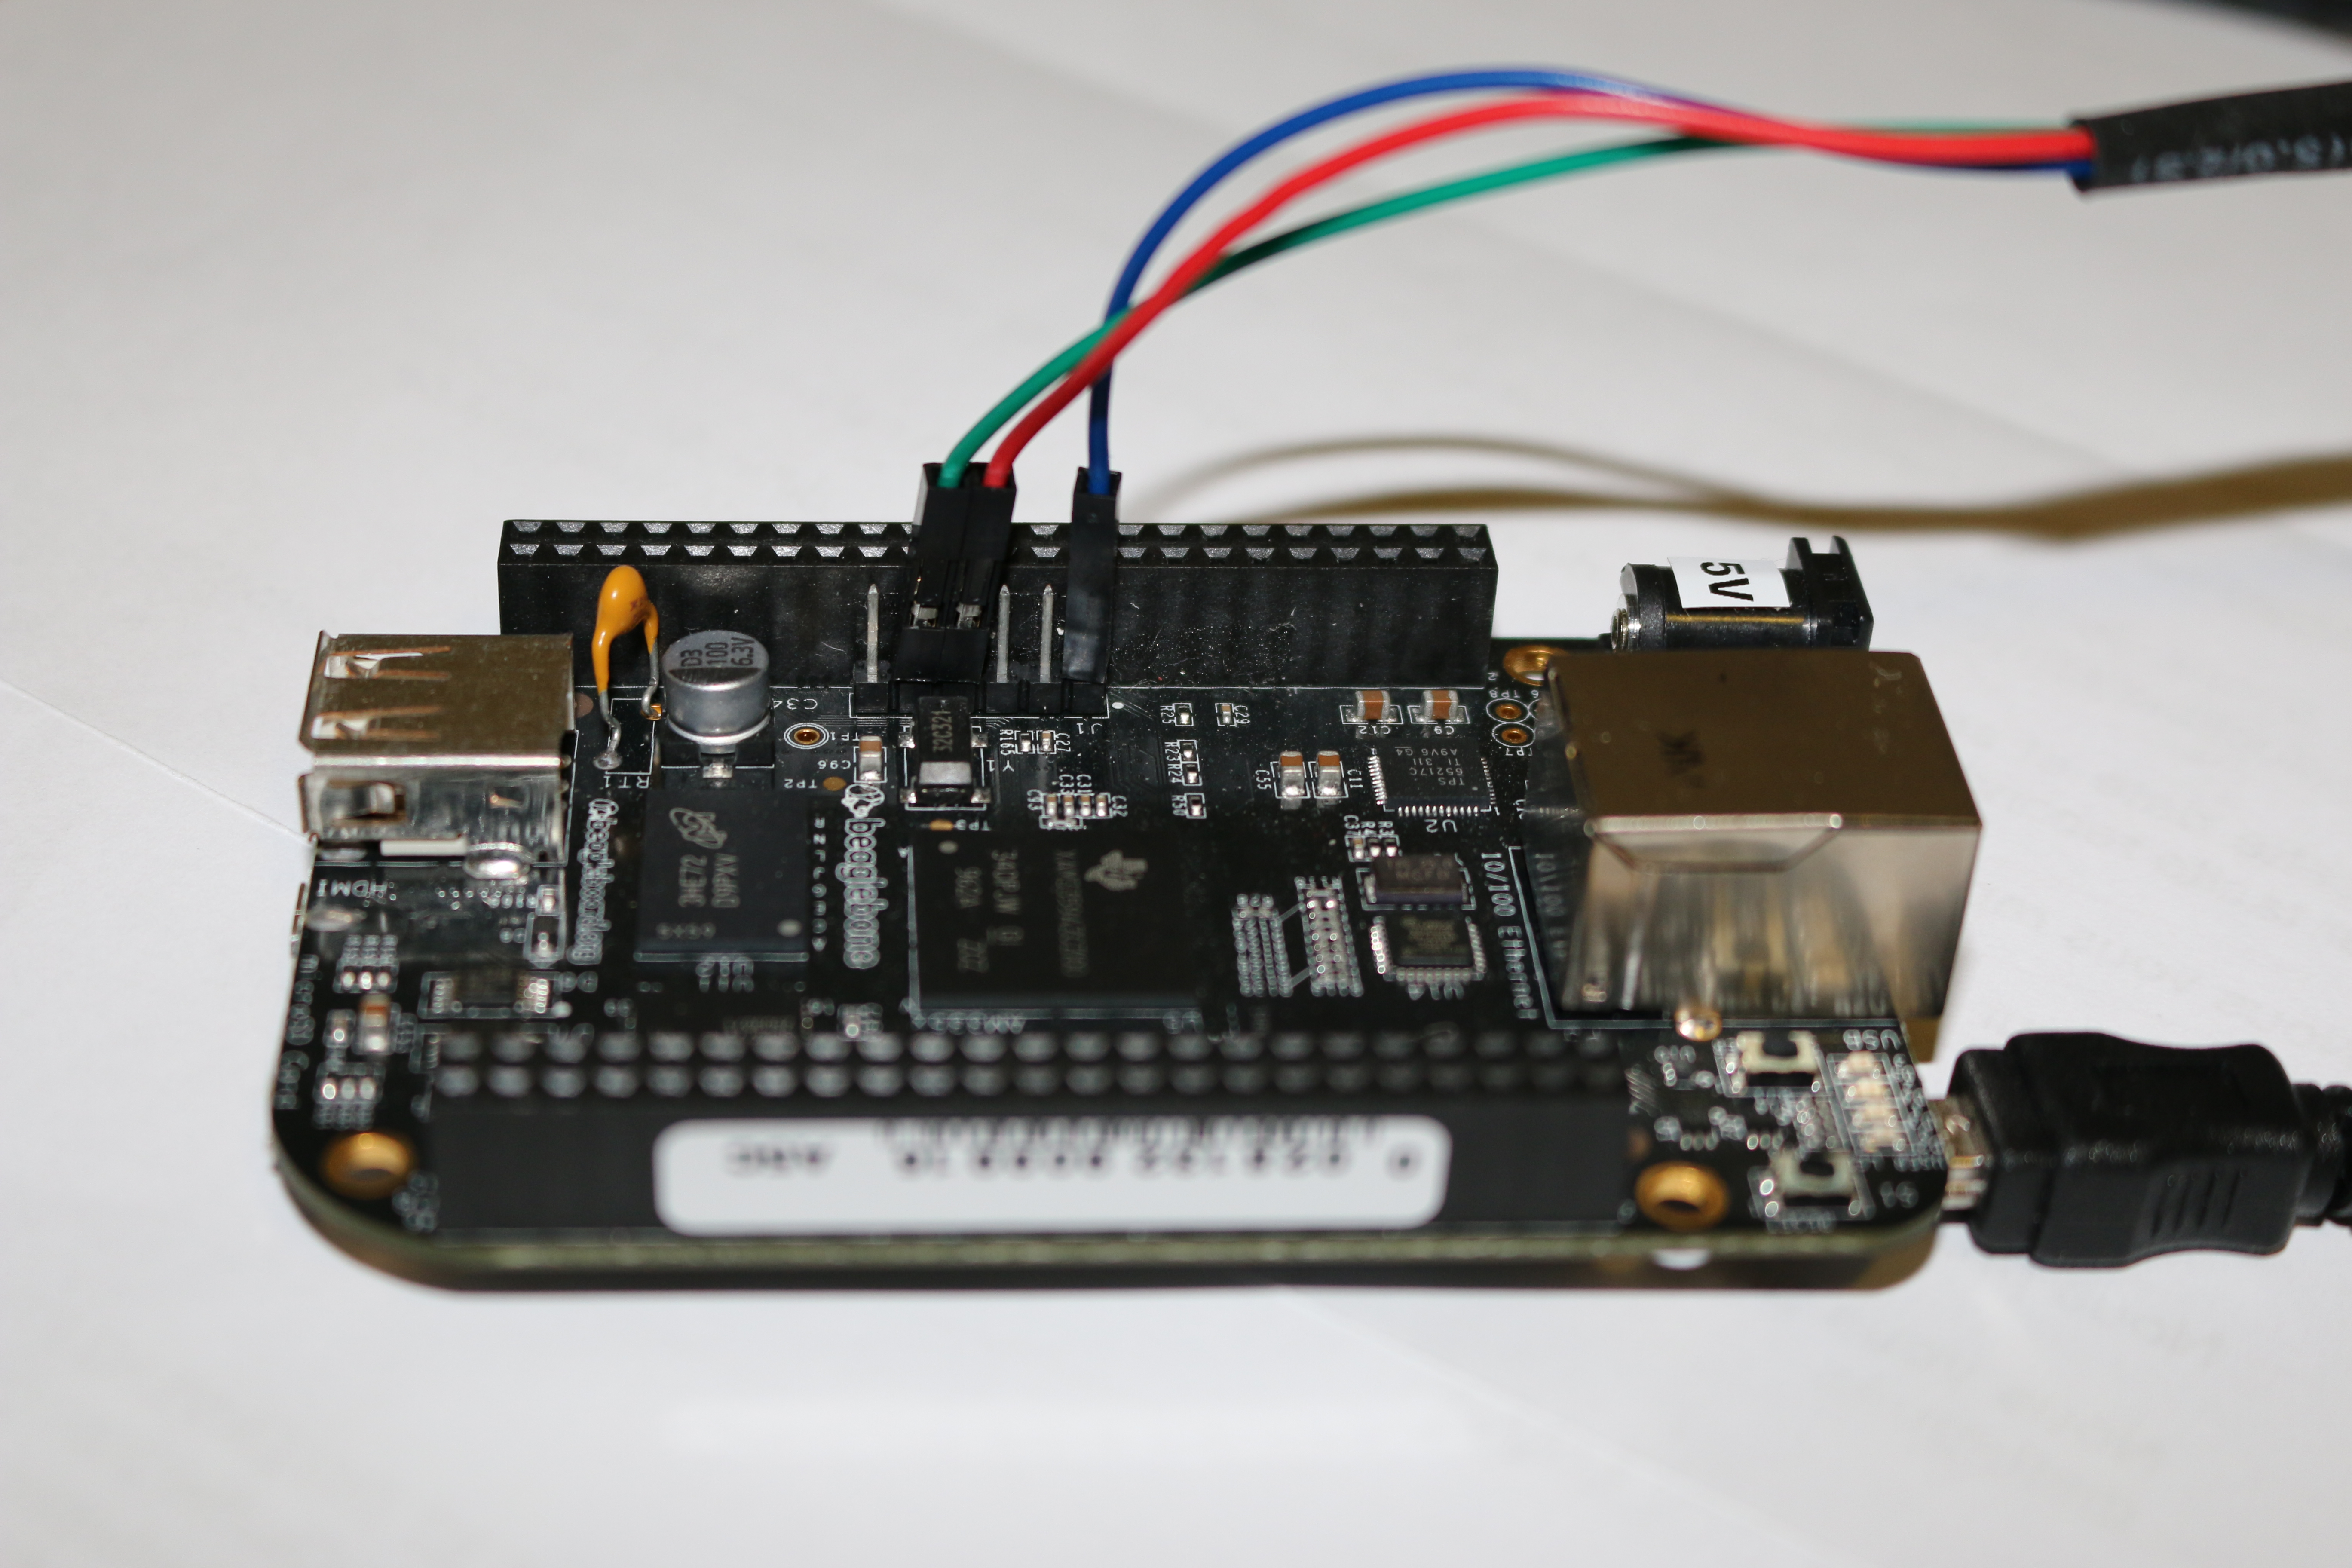
\includegraphics[width=8cm]{common/beaglebone-black-serial-connection.jpg}
\end{center}

Once the USB to Serial connector is plugged in, a new serial port
should appear: \code{/dev/ttyUSB0}.  You can also see this device
appear by looking at the output of \code{dmesg}.

To communicate with the board through the serial port, install a
serial communication program, such as \code{picocom}:

\begin{verbatim}
sudo apt install picocom
\end{verbatim}

If you run \code{ls -l /dev/ttyUSB0}, you can also see that only
\code{root} and users belonging to the \code{dialout} group have
read and write access to this file. Therefore, you need to add your user
to the \code{dialout} group:

\begin{verbatim}
sudo adduser $USER dialout
\end{verbatim}

{\bf Important}: for the group change to be effective, you have to
{\em completely log out} from your session and log in again (no need to
reboot). A workaround is to run \code{newgrp dialout}, but it is not global.
You have to run it in each terminal.

Now, you can run \code{picocom -b 115200 /dev/ttyUSB0}, to start serial
communication on \code{/dev/ttyUSB0}, with a baudrate of \code{115200}. If
you wish to exit \code{picocom}, press \code{[Ctrl][a]} followed by
\code{[Ctrl][x]}.

There should be nothing on the serial line so far, as the board is not
powered up yet.

It is now time to power up your board to its power supply through
the 5.5mm barrel jack connector (see our shopping list slide).
This is important instead of using a USB device power cable.
Otherwise you may not have enough power to drive the LCD cape
and your board may not boot any more.

See what messages you get on the serial line. You should see U-boot
start on the serial line.

\section{Bootloader interaction}

Reset your board. Press the space bar in the \code{picocom} terminal
to stop the U-boot countdown. You should then see the U-Boot prompt:

\begin{verbatim}
=>
\end{verbatim}

This step was just to check that the serial line was connected
properly. In a later lab, we will replace the existing bootloader by
a version that we compiled ourselves.

\section{Attach the LCD cape}

Switch off the board first, by pressing the \code{POWER} button until
all the LEDs go off\footnote{That's strongly recommended by the board
maker, to avoid hardware damage that can happen if the board is abruptly
switched off.}.

Now that we have successfully tested serial console, we are ready to
attach the 4.3 LCD cape provided by your instructor.

Note that if you bought your own Beagle Bone Black board, you will have
to {\bf gently} bend the serial headers using pliers, otherwise the
serial cable won't fit between the board and the cape.

Now, you can connect the LCD cape to your Bone Black board. The outline
of the Beagle Bone Black is printed on the cape to get the correct
orientation.

\begin{center}
\includegraphics[width=8cm]{labs/boot-time-board-setup/bbb-with-4dcape-43t.jpg}
\end{center}

See \url{https://resources.4dsystems.com.au/datasheets/cape/4DCAPE-43-series/}
for details about the LCD cape.
